\section*{Experimentation}

% \begin{itemize}
%     \item Dataset \& Dataset Statistics
%     \item Experimental Results based on Evaluation Metrics
%     \item Error Analysis
% \end{itemize}

This section outlines the dataset used for knowledge graph completion, presents the results of the experiments conducted using PyKEEN \textcolor{red}{and LLMs}, and includes an analysis of errors observed during model evaluation.

\subsection*{Dataset and Statistics}

\todo{REVISIT AND ADAPT THIS SECTION IF WE DECIDE TO CONTINUE WORKING WITH THIS DATASET}

The Hetionet dataset \cite{hetionet} serves as the initial foundation for this project, providing a structured biomedical knowledge graph that integrates data from various sources to represent relationships like \textit{treats}, \textit{binds}, and \textit{causes} between genes, compounds, diseases, and other biological entities. While Hetionet offers a diverse and well-documented schema, its role in this project is primarily exploratory. As we compare knowledge graph completion approaches using PyKEEN and large language models (LLMs), the dataset provides a valuable testbed for initial experiments. However, the suitability of Hetionet for future phases of the project remains under evaluation, and additional datasets may be considered as the scope of the task evolves.

Key dataset statistics are summarized in Table~\ref{tab:dataset_stats}.

\begin{table}[ht]
    \centering
    \caption{Dataset Statistics (Hetionet Subset)}
    \begin{tabular}{l c}
        \hline
        \textbf{Statistic}    & \textbf{Value} \\
        \hline
        Nodes (Entities)      & 22634          \\ % MATCH (n) RETURN count(n) AS Nodes
        Relationships (Edges) & 561721         \\ % MATCH ()-[r]->() RETURN count(r) AS Relationships
        Unique Relation Types & 10             \\ % MATCH ()-[r]->() RETURN count(DISTINCT type(r)) AS UniqueRelationTypes
        Unique Triples        & 561721         \\ % MATCH (h)-[r]->(t) RETURN count(DISTINCT [id(h), type(r), id(t)]) AS UniqueTriples
        \hline
    \end{tabular}
    \label{tab:dataset_stats}
\end{table}

\subsection*{Experimental Results and Evaluation Metrics}

To assess performance in predicting missing links using embedding models, the dataset is split into training ($80\%$), validation ($10\%$), and testing ($10\%$) sets. With this setup, as shown in Figure~\ref{fig:loss_plot}, PyKEEN's RotatE model's training loss decreases steadily, indicating successful optimization over the course of training.

\begin{figure}[ht]
    \centering
    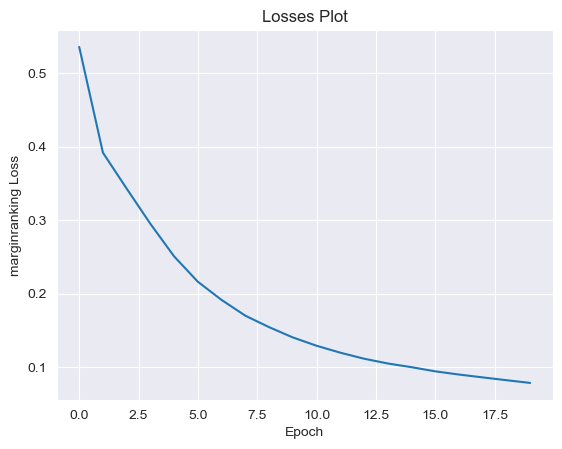
\includegraphics[width=0.6\textwidth]{images/pykeen/losses.png}
    \caption{Training loss plot for PyKEEN RotatE model over 20 epochs.}
    \label{fig:loss_plot}
\end{figure}

Evaluation is performed using standard link prediction metrics, including:

\begin{itemize}
    \item \textbf{Mean Reciprocal Rank (MRR)}: Measures the average inverse rank of the correct entity. % From 0 to 1. The higher the better
    \item \textbf{Hits@K}: Calculates the proportion of correct predictions ranked in the top $K$. % From 0 to 1. The higher the better
    \item \textbf{Mean Rank (MR)}: Provides the average rank of the correct entity. % The lower the better
\end{itemize}

The results are summarized in Table~\ref{tab:results}, comparing PyKEEN's models: RotatE\textcolor{red}{, ...}.

\begin{table}[ht]
    \centering
    \caption{Experimental Results}
    \begin{tabular}{l c c c}
        \hline
        \textbf{Model}                      & \textbf{MRR} & \textbf{Hits@10} & \textbf{MR} \\
        \hline
        RotatE                              & $0.050$      & $0.099$          & $1349.6$    \\ % Seemingly very poor results
        \textcolor{red}{TEST OTHER MODELS?} & $...$        & $...$            & $...$       \\
        \textcolor{red}{LLM (zero-shot)}    & $...$        & $...$            & $...$       \\
        \textcolor{red}{LLM (few-shot)}     & $...$        & $...$            & $...$       \\
        \textcolor{red}{LLM (RAG)}          & $...$        & $...$            & $...$       \\
        \hline
    \end{tabular}
    \label{tab:results}
\end{table}

Predicted \textit{treats} relationships for L-Asparagine were visualized (Figure~\ref{fig:predicted_treats}) suggesting potential links to diseases such as melanoma, ulcerative colitis, and coronary disease. These predictions will require further validation to confirm biological plausibility. As illustrated in Figure~\ref{fig:kg_visualization}, the graph showcases relationships between the compound L-Asparagine and breast cancer, mediated by various genes. These indirect paths offer insights into potential mechanisms that could explain the model's predictions

\begin{figure}[ht]
    \centering
    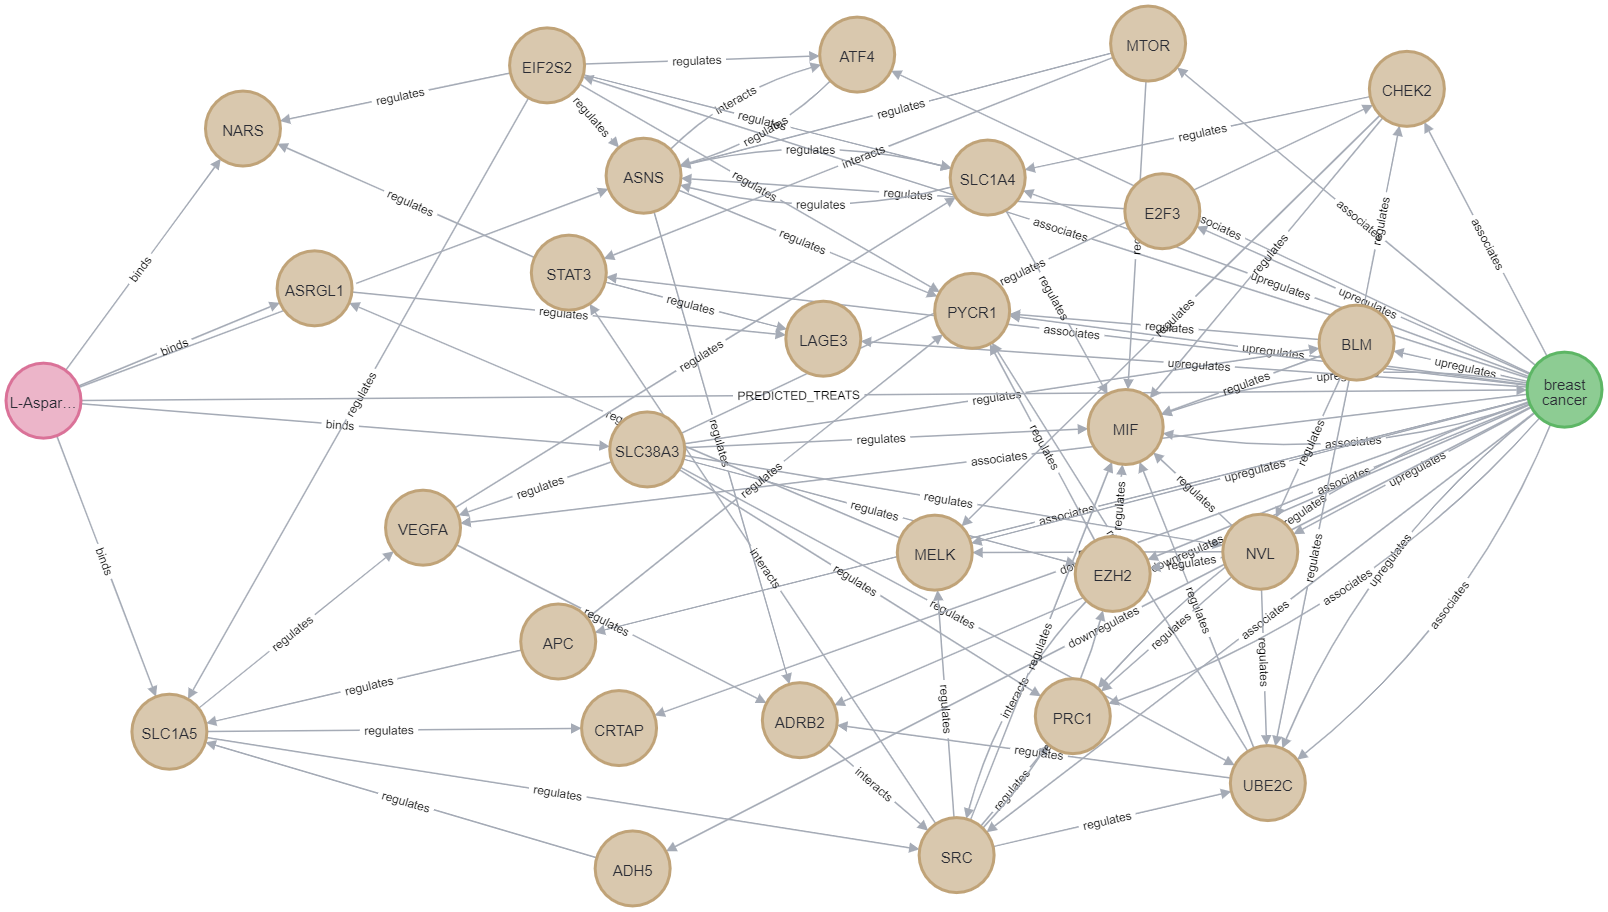
\includegraphics[width=0.8\textwidth]{images/pykeen/results.png}
    \caption{Visualization of connections between L-Asparagine, genes, and breast cancer, highlighting predicted relationships.}
    \label{fig:kg_visualization}
\end{figure}

\begin{figure}[ht]
    \centering
    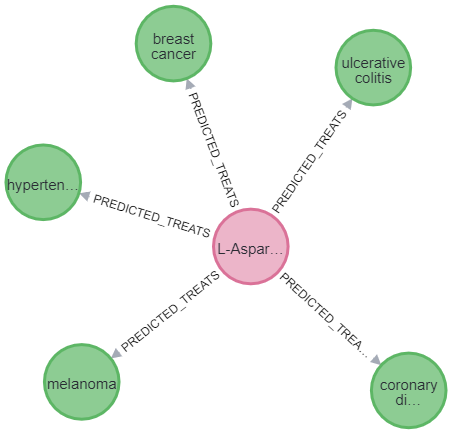
\includegraphics[width=0.45\textwidth]{images/pykeen/predicted treats.png}
    \caption{5 predicted \textit{treats} relationships for L-Asparagine.}
    \label{fig:predicted_treats}
\end{figure}

\subsection*{Error Analysis}

\todo{COMPLETE THIS SECTION}

To mitigate these errors, future work will explore: increasing the number of epochs and refining hyperparameters and incorporating negative sampling strategies to improve generalization.
